\chapter{Volba a návrh periferií}
    Tato kapitola se již věnuje návrhu konkrétních periferií, tedy jednotlivých senzorů a akčních členů. Po technické stránce jsou všechny zmíněné moduly nadstavbou pro \uv{obecný modul periferie} popsaný detailně v předešlé kapitole. Jelikož je celý systém modulární, je pravděpodobné, že postupem času bude dále rozšiřován o nové typy periferií a i v současné chvíli je jich v plánu více, než je v možnostech této práce. Pro lepší přehlednost se v tab.~\ref{tab:prehled-periferii} nachází přehled všech realizovaných i v tuto chvíli pouze plánovaných periferií.

    \begin{table}[h]
        \centering
        \caption{Přehled periferií.}
        \label{tab:prehled-periferii}
        \begin{tabular}{|l|l|l|l|l|}
            \hline
            Název & Typ & Napájení & Funkce & Realizováno \\ \hline\hline
            Sensor teploty  & S & \qty{5}{V}    & Teplota vody                       & Ano, kap.~\ref{sec:perif-sensor-teploty}  \\ \hline
            Sensor hladiny  & S & \qty{5}{V}    & Výška hladiny (spojitě + skokově)  & Ano, kap.~\ref{sec:perif-sensor-hladina}  \\ \hline
            \acs{led} osvětlení   & A & \qty{24}{V}   & Intenzita osvětlení                & Ano, kap.~\ref{sec:perif-led-osvetleni}  \\ \hline
            Sensor \acs{ph}       & S & \qty{5}{V}    & \acs{ph} vody                            & Ne, kap.~\ref{sec:perif-sensor-ph}  \\ \hline
            Topné těleso    & A & \qty{230}{V}  & Ohřev vody                         & Ano, kap.~\ref{sec:perif-230v}  \\ \hline
            Filtr vody      & A & \qty{230}{V}  & Filtrace vody                      & Ano, kap.~\ref{sec:perif-230v}  \\ \hline
            Krmítko         & A & \qty{24}{V}   & Dávkování krmiva                   & Ne  \\ \hline
            Sensor průtoku  & S & -             & Voda tekoucí filtrem               & Ne  \\ \hline
                            % & S &  &  & A  \\ \hline
                            %     & S &  &  & A  \\ \hline
                            %     & S &  &  & A  \\ \hline
                            %     & S &  &  & A  \\ \hline
                            %     & S &  &  & A  \\ \hline
                            %     & S &  &  & A  \\ \hline
                            %     & S &  &  & A  \\ \hline
                            %     & S &  &  & A  \\ \hline
                            %     & S &  &  & A  \\ \hline
            \end{tabular}
            \begin{tabular}{c}
                S = sensor, A = akční člen \\
            \end{tabular}
   
    \end{table}

\section{Senzor teploty}
\label{sec:perif-sensor-teploty}
    Cílem tohoto modulu je kontinuálně měřit teplotu vody a naměřená data poskytovat řidicí jednotce skrze sběrnici \acs{can}. Při volbě konkrétního teplotního čidla je potřeba vzít v potaz několik faktorů:
    \begin{itemize}
        \item Přesnost a rozsah
        \item Časová stálost
        \item Složitost implementace 
        \item Pouzdro určené pro ponoření do vody
        \item Cena
    \end{itemize}

    \subsection{Metody měření teploty}
        Nejčastěji používanými součástkami určenými k měření teploty jsou nepochybně termistory a termočlánky~\cite{allaboutcircuits2023tempsensors}. Termistor je rezistor vytvořen z materiálu, který mění svůj odpor v závislosti na teplotě přičemž rozlišujeme dva základní typy termistorů podle toho, zda s rostoucí teplotou jejich odpor roste (PTC termistor) anebo klesá (NTC termistor). U obou typů lze obecně říci, že závisost odporu na teplotě je značně nelineární, pro zjištění přesné teploty je tedy potřeba buďto měřená data dále zpracovat (např. mikrokontrolérem) anebo využít speciální integrovaný obvod, který výstup z připojeného termistoru linearizuje a dále propaguje buďto v analogové nebo i digitální podobě. Jelikož odpor termistoru a stejně tak i dalších součástek, potřebných k jeho zapojení, má jistou výrobní toleranci, je vhodné sensor před použitím kalibrovat.

        Princip termočlánku je odlišný, jedná se o vodivé spojení dvou kovů na kterém díky Seebeckově jevu vzniká termoelektrické napětí. Velikost tohoto napětí je daná použitými materiály a je také teplotně závislá. V praxi se používá nejčastěji několik dvojic materiálů, které svými vlastnostmi a cenou nejvíce vyhovují běžným požadavkům, ty pak získaly také své označení jako termočlánky typu J, K, T nebo E (typů existuje více, uvedeny jsou nejčastěji používané~\cite{TechieScience_Thermocouples}). Termočlánky pracují oproti ostatním senzorům s výrazně větším rozsahem teplot a mohou měřit také teploty velmi vysoké. Nevýhodou je nízké výstupní napětí, které musí být spolehlivě měřeno, tedy ideálně porovnáno s přesnou napěťovou referencí a také je potřeba, aby část zařízení, ke kterému je termočlánek připojen (tzv. studený konec), byla udržována při konstantní referenční teplotě anebo případnou změnu teploty měřila jiným způsobem a kompenzovala výpočtem~\cite{allaboutcircuits2023tempsensors,TechieScience_Thermocouples}.

        Z hlediska praxe je další často využívanou možností použití zcela integrovaného sensoru s digitálním výstupem. Pro zpracování je sice potřeba mikrokontrolér, ale tyto sensory bývají od výroby kalibrovány a také jejich zapojení je velmi jednoduché, což je výhodou.

    \subsection{Realizace sensoru}
    % TODO: Připsal bych tady krátce jak to fyzicky celé vypadá a připojuje se.
        Při porovnání uvedených metod se použití termočlánku jeví jako nevhodné, zejména kvůli náročnosti implementace, která současně navyšuje také cenu. Zbývá tedy rozhodnutí mezi termistoru a digitálním čidlem. Ve voděodolném pouzdře lze zakoupit jak několik variant termistorů, tak i digitální čidlo (zde DS18B20). Nejlevněji vychází termistor typu NTC, ale v porovnání s cenou celého zařízení je rozdíl v ceně zanedbatelný. 
        
        Pro realizaci sensoru bylo zvoleno digitální čidlo DS18B20, které narozdíl od termistoru není potřeba kalibrovat a výrobce garantuje přesnost \(\pm \qty{0.5}{\degreeCelsius}\) na celém teplotním rozsahu od \qty{-55}{\degreeCelsius} do \qty{+125}{\degreeCelsius}. Rozlišení sensoru je až 12 bitů přičemž minimální měřitelná změna teploty odpovídá \qty{0.0625}{\degreeCelsius}. Pro komunikace s čidlem se využívá protokol 1-Wire, kdy datový vodič funguje obousměrně. Pro propojení čidla s mikrokontrolérem tedy stačí využít tři vodiče a jeden pull-up rezistor, viz obr.~\ref{fig:temp-sensor-pripojeni}.


        \begin{figure}[!ht]
            \centering
            \begin{circuitikz}
                \ctikzset{resistor = european}
                % Draw the DS18B20 sensor
                \draw (0,0) node[rectangle, draw, minimum width=3cm, minimum height=5cm] (ds18b20) {};
                \node[anchor=north] at (ds18b20.south) {DS18B20};
                
                % Draw the pins on the DS18B20
                \draw (ds18b20.north east) ++(0,-0.5) coordinate (pin1);
                \draw (ds18b20.north east) ++(0,-3.0) coordinate (pin2);
                \draw (ds18b20.north east) ++(0,-4) coordinate (pin3);
                \node[left] at (pin1) {VDD};
                \node[left] at (pin2) {DATA};
                \node[left] at (pin3) {GND};
                
                % Draw the \acs{mcu}
                \draw (7,0) node[rectangle, draw, minimum width=3cm, minimum height=5cm] (mcu) {};
                \node[anchor=north] at (mcu.south) {PIC18F26};
                
                % Draw the pins on the \acs{mcu}
                \draw (mcu.north west) ++(0,-0.5) coordinate (mcupin1);
                \draw (mcu.north west) ++(0,-3.0) coordinate (mcupin2);
                \draw (mcu.north west) ++(0,-4) coordinate (mcupin3);
                \node[right] at (mcupin1) {VDD};
                \node[right] at (mcupin2) {RC7};
                \node[right] at (mcupin3) {GND};
                
                % Connect DS18B20 to \acs{mcu}
                \draw (pin1) -- (mcupin1);
                \draw (pin2) -- (mcupin2);
                \draw (pin3) -- (mcupin3);

                % Add pull-up resistor
                \draw (mcupin1) ++(-1,0) to[R, l_=4.7k, *-*] ++(0,-2.5);
            
            \end{circuitikz}
            \caption{Připojení čidla DS18B20 k \acs{mcu}.}
            \label{fig:temp-sensor-pripojeni}
        \end{figure}

\section{Senzor výšky hladiny}
\label{sec:perif-sensor-hladina}
    Voda v akváriu se průběžně odpořuje a je potřeba ji doplňovat. Účelem této periferie je průběžné monitorování hladiny akvária a upozornění uživatele na nutnost doplnění vody. Také může uživatele varovat v případě poškození nádrže a nežádoucího úniku vody do okolí. 
    K realizaci tohoto modulu jsou použity dva jednoduché sensory přičemž každý funguje na jiném principu a má tedy také odlišné přednosti a nedostatky, v kombinaci tedy zvyšují celkovou spolehlivost modulu. Oba sensory se nachází na obr.~\ref{TODO}. 

    První ze sensorů využivá k určení výšky hladiny vodivost (potažmo odpor) vody. Obsahuje dva sety vodivých plošek, které nejsou vodivě spojeny. Při ponoření měřící části do vody začne mezi ploškami procházet slabý proud, který je přibližně úměrný velikosti ponořené části. Tento proud otevírá tranzistor, na jehož výstupu pak vzniká stejnosměrné napětí v rozsahu přiloženého napájení (zde 0 až \qty{3.3}{V}). Tento signál je přiveden na pin mikrokontroleru a následně zpracován vestaveným převodníkem. PIC18F26 obsahuje integrovanou periferii ADC s rozlišením 12 bitů, teoreticky lze tedy rozlišit \num{4296} úrovní~\cite{PIC18F26Q83}. Pro převod měřené hodnoty na výšku hladiny je potřeba sensor nejprve nakalibrovat. Byla tedy změřena přibližná výstupní hodnota pro minimální a maximální měřitelné ponoření sensoru a údaj je následně mikroprocesorem převeden na procenta. Úvaj v procentech ponořené části je pro uživatele univerzálním ukazatelem nezávislým na umístení sensoru, pro měření absolutní výšky hladiny by musel uživatel v systému nastavit výšku umístění sensoru a také ji pokaždé měnit v případě změny jeho pozice.

    Druhým sensorem je jednoduchý plovák obsahující mechanický spínač, který je při ponoření do vody rozepnut. V případě poklesu hladiny pod zvolenou úroveň je pak spínač sepnut.

    Propojení mikrokontroleru s oběma sensory se nachází na obr.~\ref{fig:wl-sensor-pripojeni}.

    \begin{figure}[!ht]
        \centering
        \begin{circuitikz}
            \ctikzset{resistor = european}
            % Draw the plovak sensor
            \draw (0,0) node[anchor=south,rectangle, draw, minimum width=2cm, minimum height=3cm] (plovak) {};
            \node[anchor=north] at (plovak.south) {Plovák};
            
            % Draw the pins on the plovak
            % \draw (plovak.north east) ++(0,-0.5) coordinate (pin1);
            \draw (plovak.north east) ++(0,-1.0) coordinate (pin2);
            \draw (plovak.north east) ++(0,-2) coordinate (pin3);
            % \node[left] at (pin1) {VDD};
            \node[left] at (pin2) {};
            \node[left] at (pin3) {};
            \draw (pin3) -- ++(-0.5,0) to[spst] ++(0,1) -- (pin2);
            
            % Draw the MCU
            \draw (5,0) node[anchor=south,rectangle, draw, minimum width=4cm, minimum height=5cm] (mcu) {};
            \node[anchor=north] at (mcu.south) {PIC18F26};
            
            % Draw the pins on the MCU
            \draw (mcu.north west) ++(0,-0.5) coordinate (mcupin1);
            \draw (mcu.north west) ++(0,-3.0) coordinate (mcupin2);
            \draw (mcu.north west) ++(0,-4)   coordinate (mcupin3);
            \draw (mcu.north east) ++(0,-2)   coordinate (mcupin4);
            \draw (mcu.north east) ++(0,-3.0) coordinate (mcupin5);
            \draw (mcu.north east) ++(0,-4)   coordinate (mcupin6);
            \node[right] at (mcupin1) {VDD};
            \node[right] at (mcupin2) {RA1};
            \node[right] at (mcupin3) {GND};
            \node[left] at  (mcupin4) {VDD};
            \node[left] at  (mcupin5) {RA0};
            \node[left] at  (mcupin6) {GND};

            % Draw the Rezistivity sensor
            \draw (10,0) node[anchor=south,rectangle, draw, minimum width=2cm, minimum height=5cm] (rsens) {};
            \node[anchor=north] at (rsens.south) {PIC18F26};
            
            % Draw the pins on the rsens
            \draw (rsens.north west) ++(0,-2) coordinate (rsenspin1);
            \draw (rsens.north west) ++(0,-3.0) coordinate (rsenspin2);
            \draw (rsens.north west) ++(0,-4) coordinate   (rsenspin3);
            \node[right] at (rsenspin1) {VDD};
            \node[right] at (rsenspin2) {SENS};
            \node[right] at (rsenspin3) {GND};
            
            % Connect plovak to MCU
            \draw (mcupin1) -- ++(-1,0);
            \draw (pin2) -- (mcupin2);
            \draw (pin3) -- (mcupin3);

            % Connect rsens to MCU
            \draw (rsenspin1) -- (mcupin4);
            \draw (rsenspin2) -- (mcupin5);
            \draw (rsenspin3) -- (mcupin6);

            % Add pull-up resistor
            \draw (mcupin1) ++(-1,0) to[R, l_=100k, -*] ++(0,-2.5);
        
        \end{circuitikz}
        \caption{Připojení sensorů hladiny k MCU.}
        \label{fig:wl-sensor-pripojeni}
    \end{figure}

\section{\acs{led} osvětlení}
\label{sec:perif-led-osvetleni}

    Úkolem této periferie je zajistit osvětlení akvária a umožnit jeho ovládání. V porovnání s ostatními moduly je zapojení relativně komplexní a proto byla pro tuto periferii navržena a zhotovena vlastní \acs{dps} (fungující jako dceřinná deska, viz.~\ref{sec:modul-periferie}). Jako typ svítidla byly zvoleny \acs{led} pásky pracující s napětím \qty{12}{V}. Modul musí být schopen samostatně ovládat 2 \acs{led} pásky, kdy za pomocí regulace proudu do \acs{led} pásku nastaví intenzitu osvětlení. 

\subsection{Návrh zapojení}
    Na začátku návrhu je potřeba specifikovat si požadavky na elektrické parametry zapojení. Uvažujme délku každého pásku \(l=\qty{1}{m}\), vstupní napětí získané z konektoru D-sub \(U_{in} =\qty{24}{V}\) a výstupní napětí pro které je pásek určen \(U_{out} =\qty{12}{V}\). Pro stanovení maximálního proudu bylo vycházeno z údajů na e-shopu \acs{led} Solution~\cite{eshop-ledsolution-svetlo}, kdy nejvýkonější nabízený \acs{led} pásek pro dané napětí má příkon \(P_{i}= \qty{20}{W/m}\). Pak každý kanál musí být schopen dodat proud odpovídající nejnáročnějšímu scénáři:
    \begin{equation}  
        I_{max} = \frac{P_{i}\cdot l }{U_{out}} = \frac{20\cdot 1 }{12} = \qty{1.66}{A}
    \end{equation}

    Jelikož se jedná o dceřinnou desku pro obecný modul, rozměr výsledné \acs{dps} je omezen a část plochy je navíc využita konektory pro vsazení do obecného modulu. Je tedy potřeba zvolit co nejvíce integrované řešení, které současně slibuje dobrou účinnost a tedy co nejnižší ohřev zařízení během provozu.

    Pro řízení \acs{led} osvětlení je často používán proudový zdroj, který umožňuje lineárně regulovat výstupní proud a tím i intenzitu osvětlení. Na trhu existuje opět celá řada čipů určena přímo k ovládání \acs{led} pásků~\cite{TI_\acs{led}_Drivers}, problém je zde ale v tom, že uživatel velmi pravděpodobně připojí pásek s nižším, předem neznámým příkonem. Maximální proud je tedy specifický danému \acs{led} pásku a proudový zdroj by musel zároveň spolehlivě zaručit, že nebude překročeno napětí \(U_{out} =\qty{12}{V} \).

    Touto funkcí většina čipů nedisponuje a pokud ano, nejsou dostatečně integrované pro použití v této aplikaci. Po důkladné rešerši a několika iteracích návrhu se nakonec jeví jako nejlepší možnost použití napěťového měniče typu buck spolu se zesilovačem pro snímání proudu. Snímaný proud je následně zpracován mikrokontrolérem a jsou upraveny poměry ve zpětné vazbě měniče, aby napětí odpovídalo požadovanému proudu.

    \begin{figure}[h!]
        \centering
        % trim=left bottom right top
        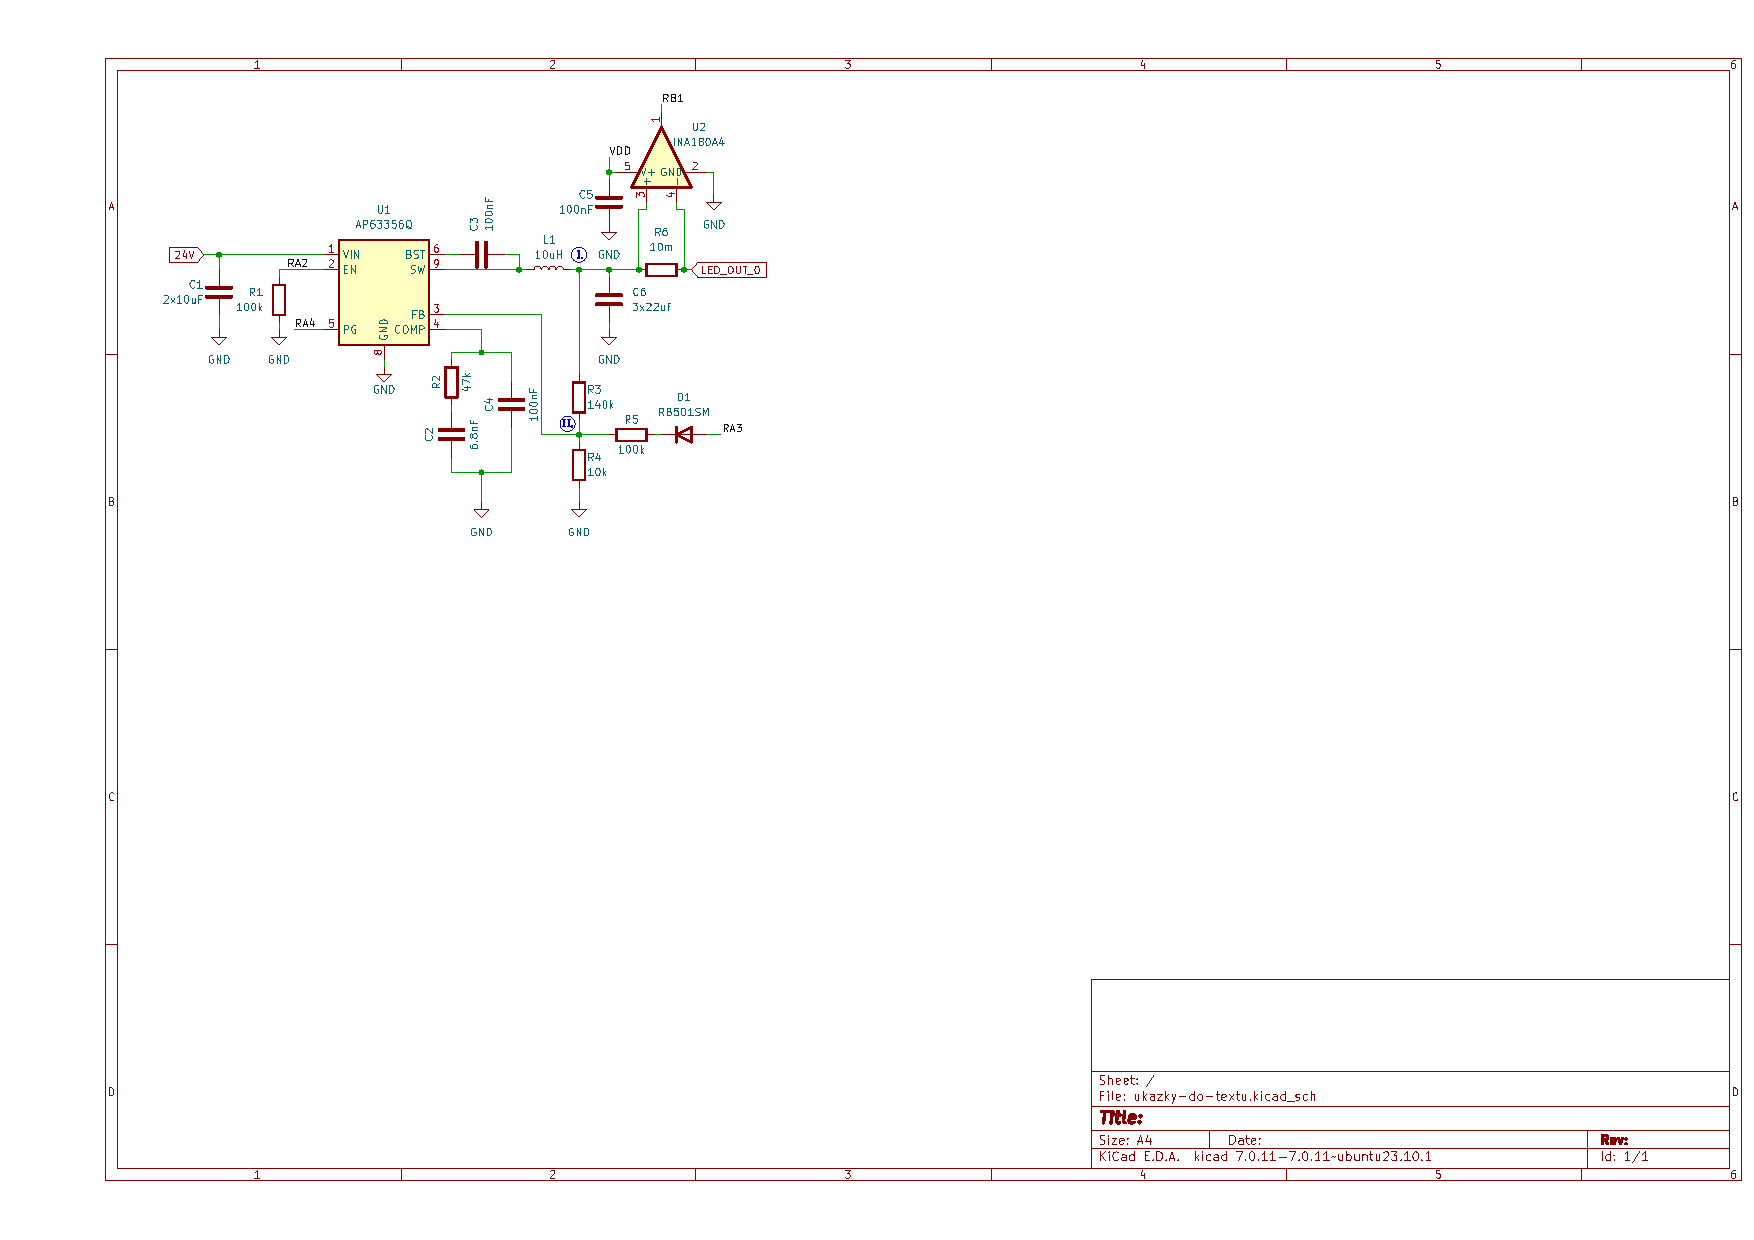
\includegraphics
        [
            width=\textwidth, 
            page=1, 
            trim=2.5cm 11.5cm 16cm 1.5cm, 
            clip
        ]{obrazky/exportovane/ukazky-do-textu.pdf}
        \caption{Zjednodušené schéma ovladače \acs{led}. Vytvořeno v~KiCad 7.0.}
        \label{fig:led-board-simp-schema}
    \end{figure}

    
\subsubsection{Popis schématu a výpočty hodnot součástek}
    Zjednodušené schéma pro jeden ovládaný kanál se nachází na obr.~\ref{fig:led-board-simp-schema}, při výpočtech bude použito označení součástek z tohoto schématu. Úplné schéma modulu pak lze nalézt v příloze~\ref{priloha:schema-led-board}.

    Jako buck kontrolér je zvolen čip AP63356Q vyvinutý společností Diodes incorporated, jedná se o úspornou a velmi malou součástku, která v sobě integruje oba potřebné MOSFET tranzistory a spíná s pevně danou frekvencí \(f_{SW}=\qty{450}{kHz} \) ~\cite{Diodes_AP63356Q}. Pro snímání proudu poslouží čip INA180A4 firmy Texas Instruments~\cite{TI_INA180A4}.

    Z obrázku je vidět, že pro ovládání jednoho kanálu \acs{led} pásků jsou využity 4 piny \acs{mcu}. RA4 a RB1 fungují jako vstupy, RA2 a RA3 pak jako výstupy. Rezistor \(R_{1}\) drží buck měnič ve vypnutém stavu, dokud mikrokontrolér nenastaví hodnotu pinu RA2 na logickou 1. Pin RA4 je pak čipem (U1) stažen k zemi vždy, když na výstupu není odpovídající nastavené napětí.  
    
    Nastavení výstupního napětí měniče je dosaženo za pomoci zpětnovazební smyčky mezi výstupním uzlem (I.) a zpětnovazebním pinem FB (uzel II.). V uzlu II. je drženo konstantní napětí \qty{0.8}{V}~\cite{Diodes_AP63356Q}, poměrem rezistorů R3 a R4 je pak definováno výstupní napětí. Zvolíme hodnotu odporu \(R_{4} = \qty{10}{k\ohm}\), pro maximální požadované napětí \(U_{outMAX} = \qty{12}{V}\) platí:
    \begin{equation}
        R_{3} = R_{4}\cdot \left(\frac{U_{outMAX} }{\num{0.8}}-1\right) = \qty{10}{k}\cdot \left(\frac{12}{\num{0.8}}-1\right) = \qty{140}{k\ohm}
    \end{equation} 
    Na pin RA3 mikrokontroléru je přivedeno analogové napětí z periferie \acs{dac} popř. \acs{pwm} signál. Skrze rezistor R5 (a ochrannou diodu) pak teče proud do rezistoru R4, úbytek napětí na tomto rezistoru je ale konstantní (\qty{0.8}{V}) a tedy je konstantní i proud rezistorem. Z prvního Kirchhoffova zákona pak víme, že proud rezistorem R3 klesne o hodnotu proudu dodanou z pinu RA3, tím klesne také napětí na výstupu měniče a dojde ke ztlumení jasu \acs{led} pásku. Citlivost (nebo také rozsah) změny je definována hodnotou R5, snížením jeho hodnoty lze dosáhnout na výstupu ještě nižšího napětí. Pro hodnotu \(R_{5} = \qty{100}{k\ohm}\) zobrazenou ve schématu lze nejnižší možné napětí vypočítat následovně:
    \begin{equation}
        U_{outMIN} = \num{0.8}+R_{3} \cdot I_{3} = \num{0.8}+R_{3} \cdot \left(\frac{\num{0.8}}{R_{4}} - \frac{U_{VDD} - U_{D1}}{R_{4}+R_{5}} \right) 
    \end{equation}  
    Kdy \(U_{VDD} = \qty{3.3}{V}\) je maximální napětí pinu RA3 a \(U_{D1}=\qty{0.35}{V} \) je prahové napětí zvolené diody. Po dosazení získáme:
    \begin{equation}
        U_{outMIN} = \num{0.8}+\qty{140}{k} \cdot \left(\frac{\num{0.8}}{\qty{10}{k}} - \frac{\num{3.3} - \num{0.35}}{\qty{10}{k}+\qty{100}{k}} \right) = \qty{8.25}{V}
    \end{equation}  
    Toto napětí by mělo být dostatečně nízké k úplnému zhasnutí \acs{led} pásku.

    TODO: Kompenzace

    V dalším kroku je stanovena hodnota induktoru L1. Výrobce doporučuje zvolit zvlnění proudu induktorem (ripple) \(\Delta I_{L}  \) jako 30 až \qty{50}{\percent} maximálního odběru. Pro výpočet induktoru je uvažován maximální povolený proud čipem, tím je zajištěno, že čip bude fungovat i po překročení maximálního očekávaného proudu \(I_{max} = \qty{1.66}{A} \). Při zvolení střední hodnoty \qty{40}{\percent} získáme:
    \begin{equation}
        \Delta I_{L} = \num{0.4}\cdot I_{IC-max} = \num{0.4} \cdot  \num{3.5} = \qty{1.4}{A}
    \end{equation}
    Odpovídající hodnota indukčnosti je vypočtena následujícím vztahem:
    \begin{equation}
        L_{1} = \frac{U_{outMAX}\cdot (U_{in} -U_{outMAX} ) }{U_{in} \cdot \Delta I_{L}\cdot f_{SW}  }
    \end{equation}
    Po dosazení získáme:
    \begin{equation}
        L_{1} = \frac{12\cdot (24 -12 ) }{24 \cdot \num{1.4}\cdot \qty{450}{k}  } = \qty{9.52}{\micro H}
    \end{equation}
    Zvolíme nejbližší běžně používanou hodnotu \(L_{1} = \qty{10}{\micro H}\). 

    Pro vstupní (C1) a výstupní (C6) kapacitu použijeme hodnoty doporučené výrobcem, stejně tak pro bootstrap kondenzátor C3. 
    
    Poslední součástkou zůstává měřicí rezistor R6. Tímto rezistorem protéká celý výstupní proud měniče, v rámci minimalizace ztrátového výkonu by měl mít tedy co nejmenší odpor. Musíme ovšem také brát v potaz rozsah měřicího zesilovače INA180A4. Tato součástka se vyrábí v několika variantách, byla zvolena varianta s nejvyšším ziskem \(G_{INA}=200 \) pro zachování co nejnižší hodnoty rezistoru, výstupní napětí zesilovače je v rozsahu 0 až \qty{3.3}{V} (VDD mikrokontroléru).
    Při maximálním očekávaném proudu chceme dosáhnout horní hranice rozsahu zesilovače, z této podmínky vyplývá vztah pro výpočet odporu rezirtoru R6:
    \begin{equation}
        R_{6} = \frac{U_{VDD}}{I_{max} \cdot G_{INA} } = \frac{\num{3.3}}{\num{1.66}\cdot 200} = \qty{9.94}{m\ohm}
    \end{equation} 
    Zvolíme blízkou hodnotu \(R_{6} \) = \qty{10}{m\ohm}.


\subsubsection{Očekávané parametry}
    Pro výpočet výstupního zvlnění (v uzlu I.) chybí údaj o ekvivalentním sériovém odporu (ESR) výstupních kondenzátorů (C6), který výrobce neuvádí. Vyjdeme tedy z typické hodnoty pro keramický kondenzátor \(ESR=\qty{15}{m\ohm}\)~\cite{wikipedia2024esr}, kdy počítáme s paralelní kombinací tří kondenzátorů.
    Očekávané výstupní zvlnění je tedy přibližně:
    \begin{equation}
        \Delta U_{out} = \Delta I_{L} \cdot  \left(\frac{ESR}{3}+\frac{1}{8\cdot f_{SW} \cdot C_{6} }\right) 
    \end{equation} 
    \begin{equation}
        \Delta U_{out} = \num{1.4} \cdot  \left(\frac{\qty{15}{m}}{3}+\frac{1}{8\cdot \qty{450}{k} \cdot 3\cdot \qty{22}{\micro\,} }\right)  = \qty{13}{mV}
    \end{equation} 

    \textit{TODO: Zde velký question: Pokusit se o přesnější výpočet ztrát a účinnosti nebo se odkázat na kalkulačku výrobce, která stejně bude nejpřesnější?}
    % Jestli chceš tak nebo tak je to celkem jedno. Nicméně kalkulačka výrobce vůbec nemusí být nejpřesnější. Naopak výrobci kolikrát kecají a ukáží ti lepší výsledek.

\subsection{Tvorba \acs{dps}}
    Jak již bylo zmíněno v úvodu kapitoly, jedná se o dceřinnou desku pro obecný modul periferie, čímž jsou jasně určeny její maximální rozměry. Stejně jako u předešlých návrhů, i zde je použita čtyřvrstvá struktura viz obr.~\ref{fig:ridici-jednotka-stackup-dps}. Vizualizace návrhu se nachází na obr.~\ref{fig:perif-led-dps} spolu s ukázkou sesazení s obecným modulem periferie. 


    \begin{figure}[!ht]
        \centering
        \begin{tikzpicture}
            % Include the image
            \node[anchor=south west,inner sep=0] (image) at (0,0) {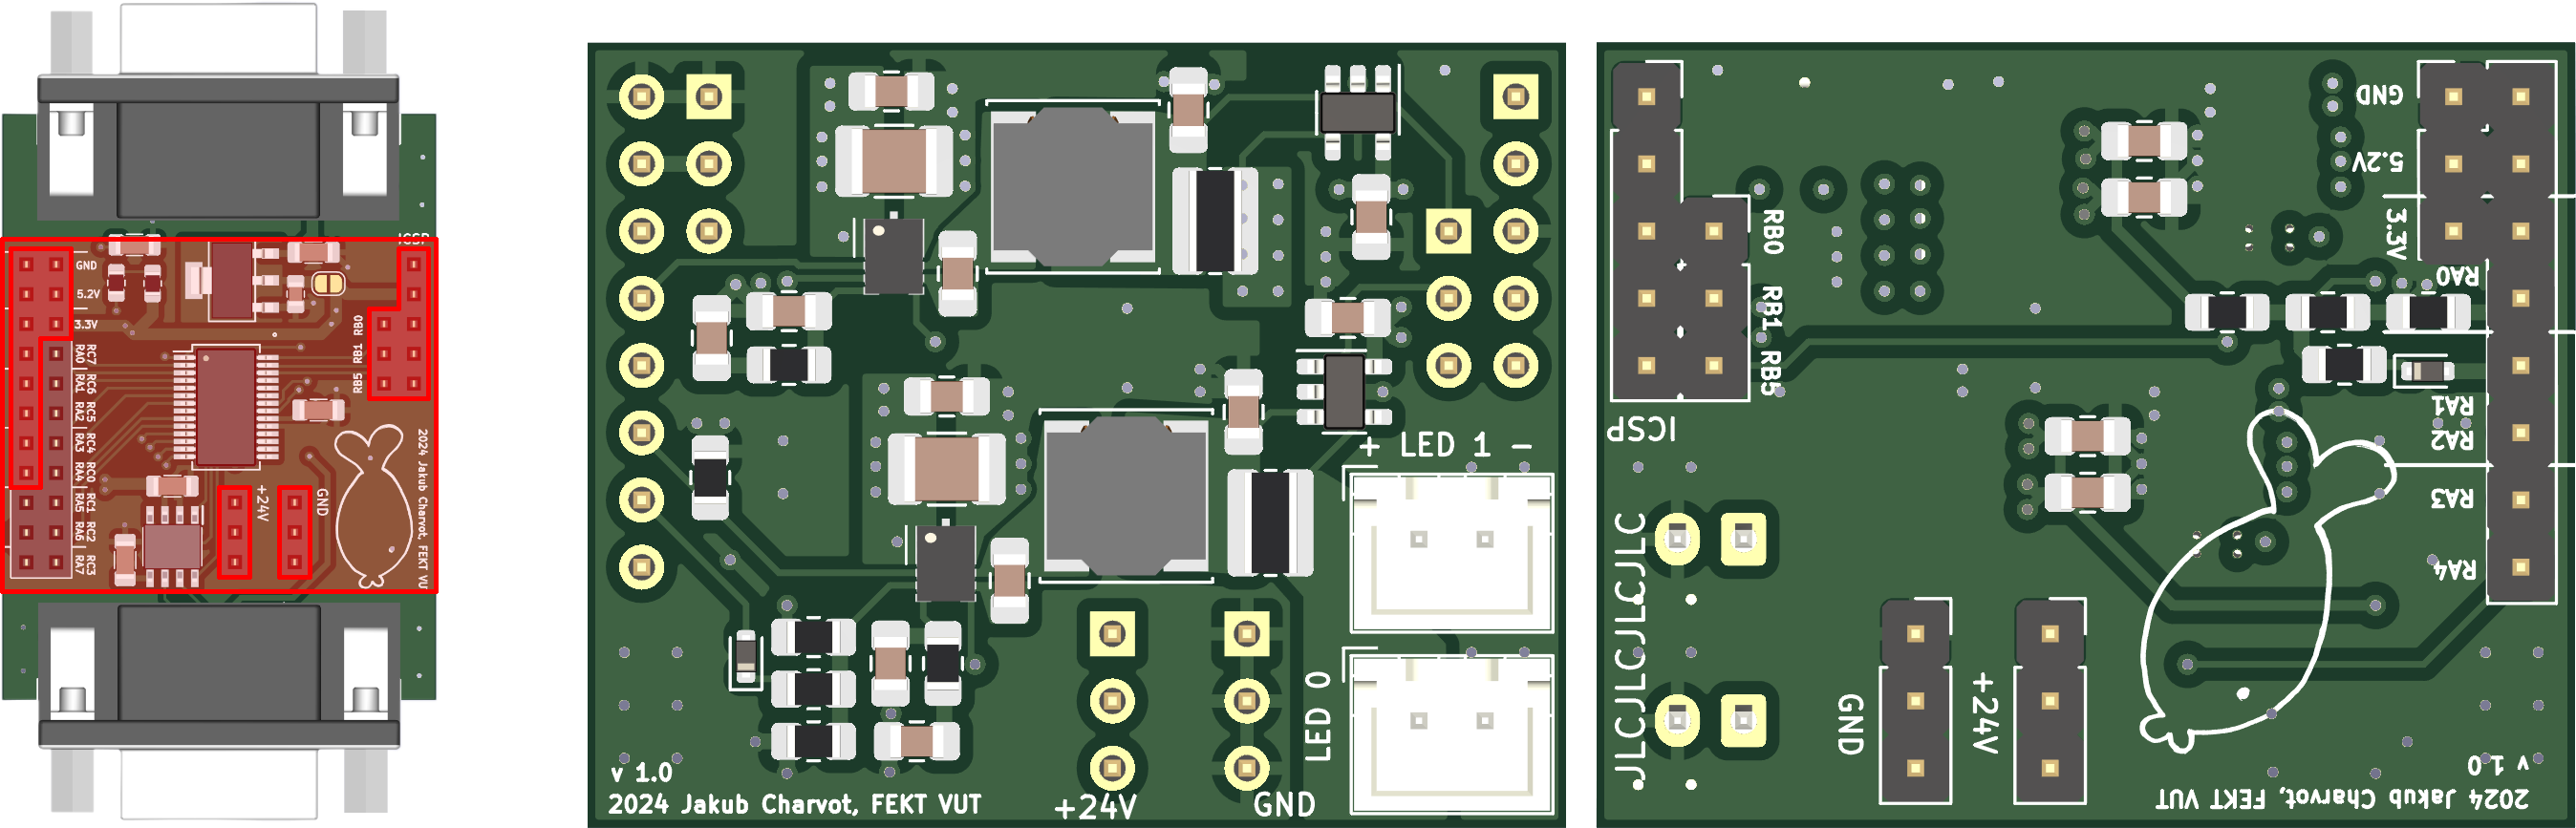
\includegraphics[width=0.8\textwidth]{obrazky/dps/ledboard-combined.png}};
            
            \draw[dashed] (10.1,0.02) -- (12.5,0.02);
            \draw[<->,thick] (12.5,0.02) -- (12.5,3.66);
            \draw[dashed] (12.5,3.66) -- (10.1,3.66);
            \node[anchor=west] at (12.5,1.83)  {\qty{36}{mm}};

            \draw[dashed] (2.75,0.02) -- (2.75,-0.5);
            \draw[<->,thick] (2.75,-0.6) -- (7.3,-0.6);
            \draw[dashed] (7.3,-0.6) -- (7.3,0.02);
            \node[anchor=south] at (5,-0.6)  {\qty{57}{mm}};

            \draw[dashed,thick,color=red] (2.75,0.02) -- (2.05,1.1);
            \draw[dashed,thick,color=red] (2.75,3.66) -- (2.05,2.7);
        \end{tikzpicture}
        \caption{Vizualizace \acs{dps} periferie \acs{led} osvětlení.}
        \label{fig:perif-led-dps}
    \end{figure}

    Za účelem zvětšení plochy pro umístění součástek byly z konektorů obecného modulu vyvedeny pouze některé piny, i přesto bylo nakonec potřeba umístit komponenty také na spodní stranu \acs{dps}. Rozmístění součástek je obdobné pro oba měniče napětí a respektuje doporučení výrobce a tedy i obecná pravidla pro návrh měničů napětí~\cite{Diodes_AP63356Q}. Je kladen důraz na to, aby smyčka ze spínacího uzlu přes výstupní kapacitu a zem zpět do kontroléru byla co nejkratší a vedena za pomoci polygonů. Stejně tak vstupní kapacitor je umístěn přímo vedle vstupních pinů kontroléru.
    




\section{Senzor \acs{ph}}
\label{sec:perif-sensor-ph}
Kapitola~\ref{sec:monitorovani} stručně popisuje význam měření pH vody v akváriu. Ačkoliv informace o pH vody může být velmi užitečná, lze konstatovat, že kontinální měření této veličiny není pro provoz akvária nutností. Vývoj této periferie proto neměl v rámci práce nejvyšší prioritu a z důvodu nedostatku času nakonec nebyla realizována.

Nejjednodušším způsobem nepřetržitého měření je použití pH sondy. V rámci této práce byla zvolena elektrochemická sonda E201, kterou je možno vidět na obr.~\ref{fig:obrazky-foto-ph_sonda-jpeg}. Sonda se kládá ze dvou elektrod, referenční a měřicí. Měřicí elektroda je umístěna ve skleněném pouzdře opatřeném iontově sensitivní úpravou. Elektroda reaguje na kationty vodíku H+, které přímo souvisí s pH měřeného roztoku. Princip měření je potenciometrický. Referenční elektroda generuje stabilní potenciál, naopak na elektrodě měřicí vzniká potenciál závislý na pH roztoku. Potenciálový rozdíl je pak měřitelný dalšími obvody. Pro korektní převod měřené hodnoty je potřeba sensor kalibrovat. Jednoduchou kalibraci lze provést vložením sondy do dvou roztoků známého pH a následným proložením měřených hodnot kalibrační přímkou. K vytvoření kalibračních roztoků se využívá speciálních prášků, které lze zakoupit spolu se samotnou sondou.

\begin{figure}[h!]
    \centering
    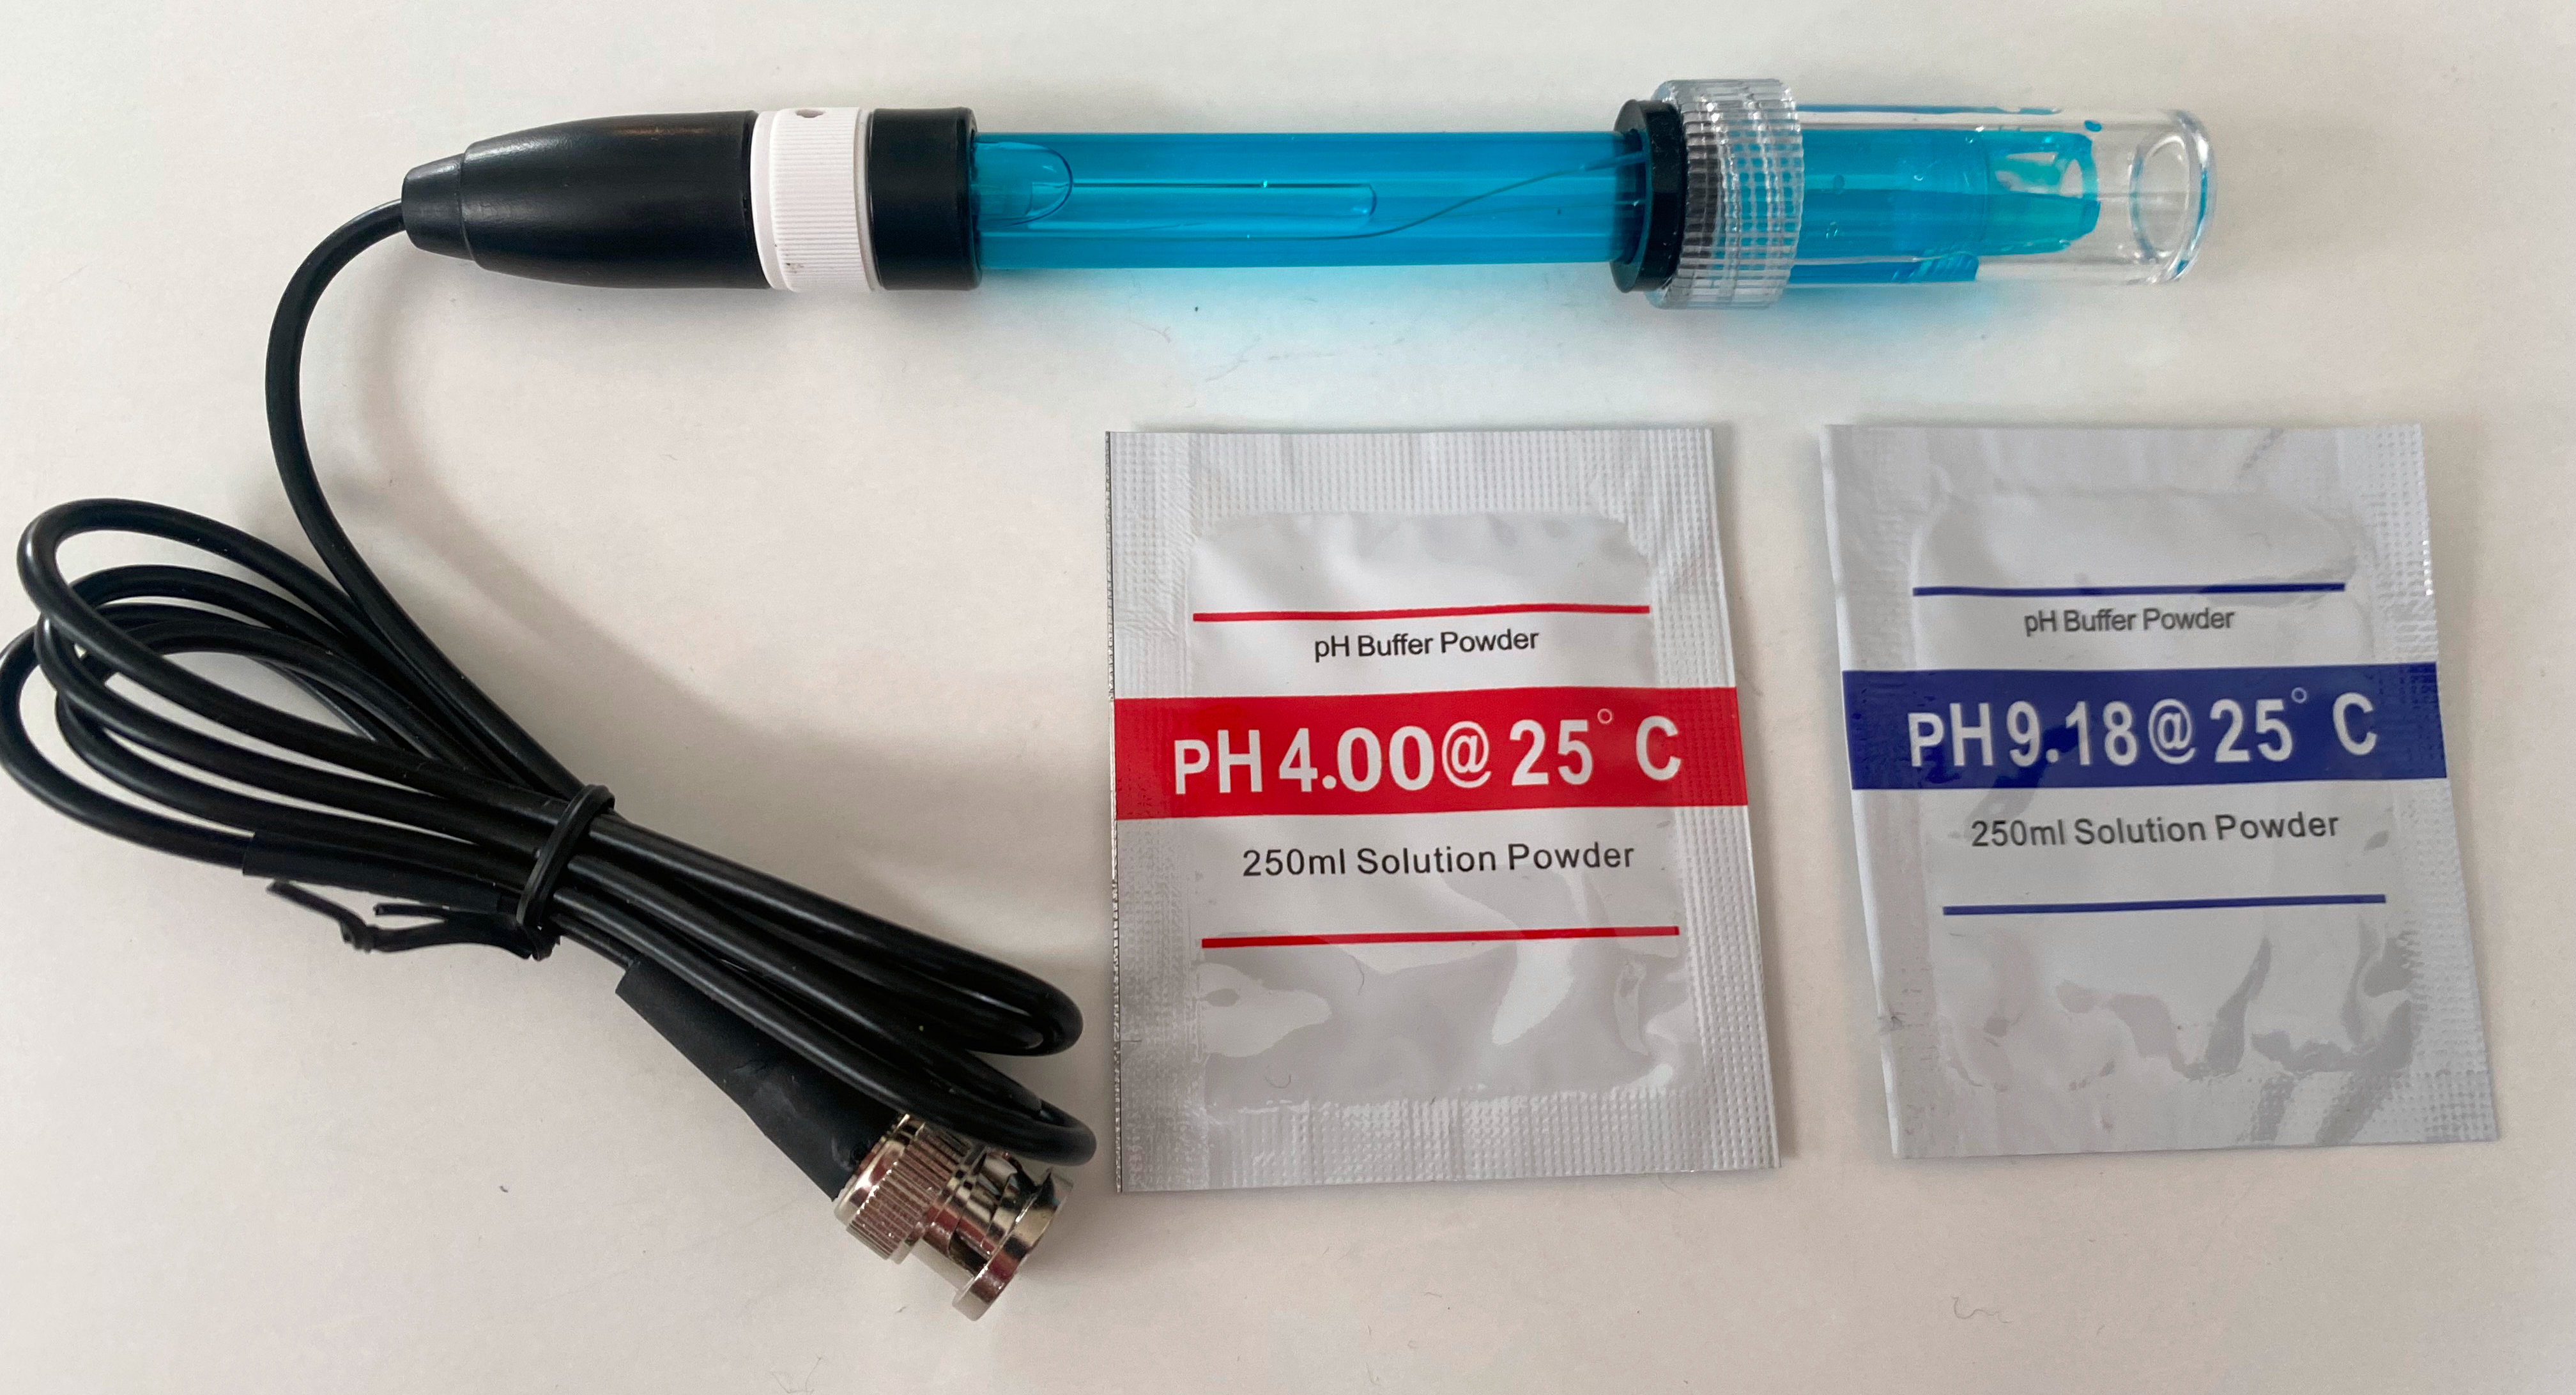
\includegraphics[width=0.8\textwidth]{obrazky/foto/ph_sonda.jpeg}
    \caption{pH sonda E201 spolu s kalibračními prášky.}
    \label{fig:obrazky-foto-ph_sonda-jpeg}
\end{figure}

Z hlediska mikrokontroléru je zapotřebí periferie ADC (analogově digitální převodník). Použitý PIC18F26 je vybaven převodníkem s rozlišením  12 bitů, což je pro danou aplikaci více než dostatečné. Aby samotný sensor nebyl příliš proudově zatížen, bude pravděpodobně nutné přidat mezi sensor a mikrokontrolér ještě operační zesilovač. 

\section{Ovládání 230V periferií}
\label{sec:perif-230v}
Jak vyplývá z~požadavků zařízení a přehledu používané akvaristické techniky, pro automatizovaný provoz akvária je nutné umožnit řídicí jednotce ovládat několik okruhů se síťovým napětím a spínat tak zvlášť zakoupené hotové spotřebiče pracující s~tímto napětím. Jedná se typicky o~ohřev vody, filtraci, popř. některé druhy osvětlení. 

\begin{figure}[h!]
    \centering
    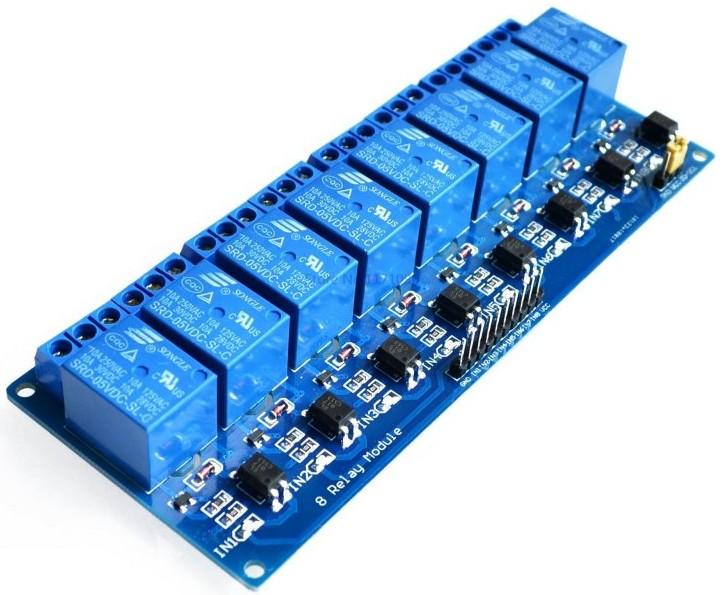
\includegraphics[width=0.6\textwidth]{obrazky/230/rele.jpg}
    \caption{TODO vyměnit: Relé modul, ilustrační foto. Převzato z~\cite{eshop-laskakit-rele}.}
    \label{fig:obrazky-230-rele-jpg}
\end{figure}


Aby uživatel mohl spínaná zařízení bezpěčně připojit bez nutnosti odborné způsobilosti, nachází se na hlavním šasi zařízení čtyři standartní zásuvky (typ E) s~jednofázovým napětím \qty{230}{V}. Fázové vodiče jsou uvnitř zařízení přerušeny spínacími relé. Je použit předpřipravený modul disponující osmi relé~\cite{eshop-laskakit-rele}, čtyři z nich tedy zůstanou nevyužité a slouží jako rezerva pro případ poškození některého z~používaných relé nebo při potřebě budoucího rozšíření o~další zásuvky. 

Z~důvodu nedostatku pinů na mikrokontroléru řídicí jednotky (ESP32) je k~relé modulu připojen ještě jeden externí modul a to expandér \acs{gpio} pinů komunikující přes sběrnici \acs{i2c}~\cite{eshop-laskakit-expander}. Z~pohledu mikrokontroléru jsou tak všechny zásuvky ovládány pomocí dvou \acs{gpio} pinů (\acs{sda}, \acs{scl}), které je navíc možné dále využít pro připojení jiných periferií jako např. O\acs{led} displaje pro zobrazení stavu zařízení.

Relé na použitém modulu potřebuje pro spolehlivé sepnutí napětí alespoň \qty{5}{V}, logické signály řídicí jednotky ale pracují s napětím pouze \qty{3.3}{V}. Ze schématu na obr.~\ref{fig:relay-board-simp-schema} je vidět, že použitý relé modul je spínán signálem logické nuly, tímto způsobem je problém s rozdílnou úrovní napájení elegantně vyřešen. 

\begin{figure}[h!]
    \centering
    % trim=left bottom right top
    \includegraphics
    [
        width=\textwidth, 
        page=3, 
        trim=2.5cm 14.5cm 18cm 1.5cm, 
        clip
    ]{obrazky/exportovane/ukazky-do-textu.pdf}
    \caption{Schéma jednoho kanálu relé modulu. Vytvořeno v~KiCad 7.0.}
    \label{fig:relay-board-simp-schema}
\end{figure}

Do budoucna by bylo možným zlepšením a rozšířením této práce zahrnutí obou zmíněných modulů přímo na \acs{dps} řídicí jednotky. 


